\begin{figure}[t]
\centering
\begin{minipage}[c]{0.35\textwidth}
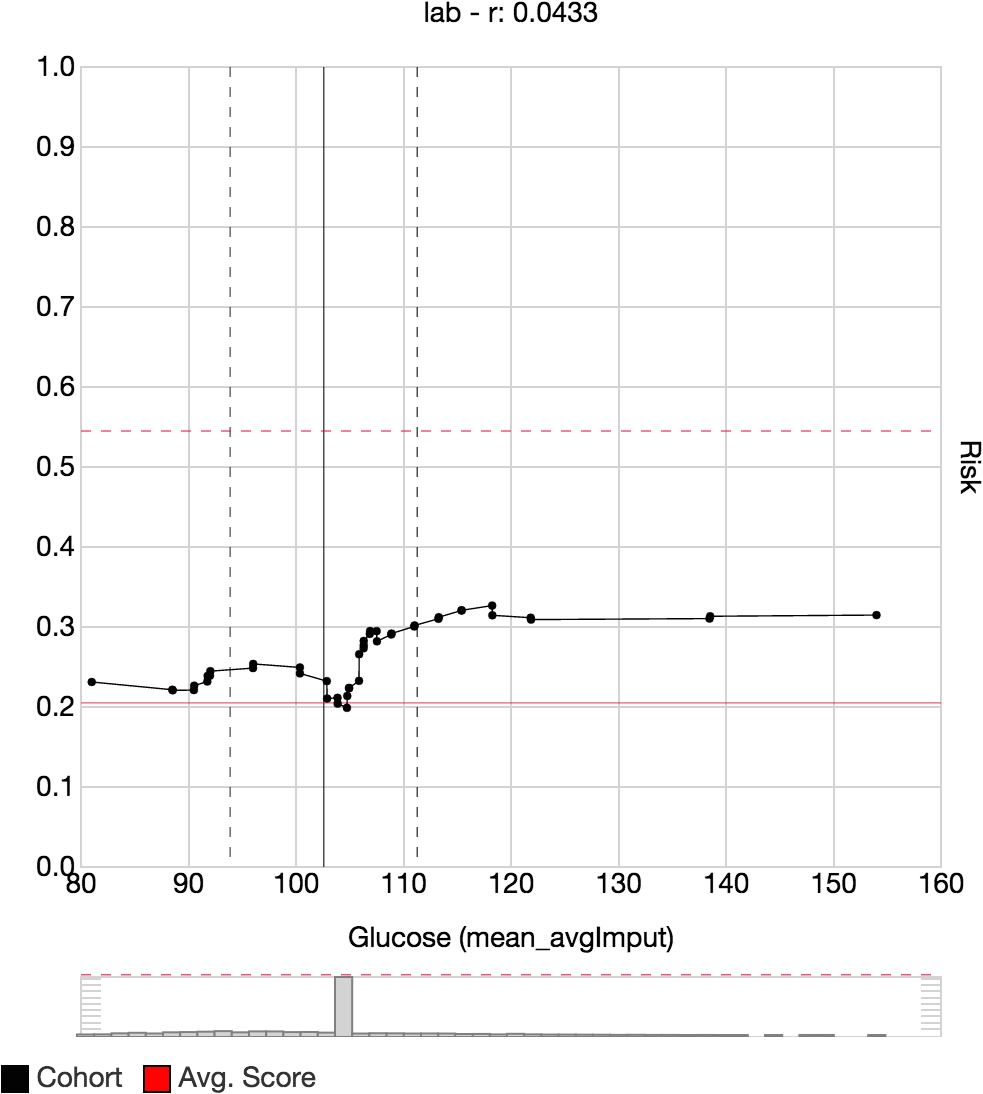
\includegraphics[width=\linewidth]{figs/prospector/debug} % 19.5
\end{minipage}\hfill
\begin{minipage}[c]{0.6\textwidth}
\caption{
Debugging model performance using partial dependence.
Instead of a direct relationship between higher Glucose lab values (x-axis) and higher risk scores (y-axis)
the model predicts a low risk for average Glucose lab values.
The histogram below the plot, showing the distribution of the values found in the input data, indicates that most patients have the average value.
% As can be seen in the distribution of the values as seen in the data set (histogram below the plot) most patients have the average value.
Since missing values are imputed using the average Glucose value the valley in the plot
can be explained by the outcome independence of this value due to the high number of missing values.
}
\label{figs:prospector_debug}
\end{minipage}
\end{figure}